%% Auto-generated by scripts/make_figures.py - do not edit by hand.
%% \input this file; PDFs live in the figures/ directory.

\begin{figure}[t]
  \centering
  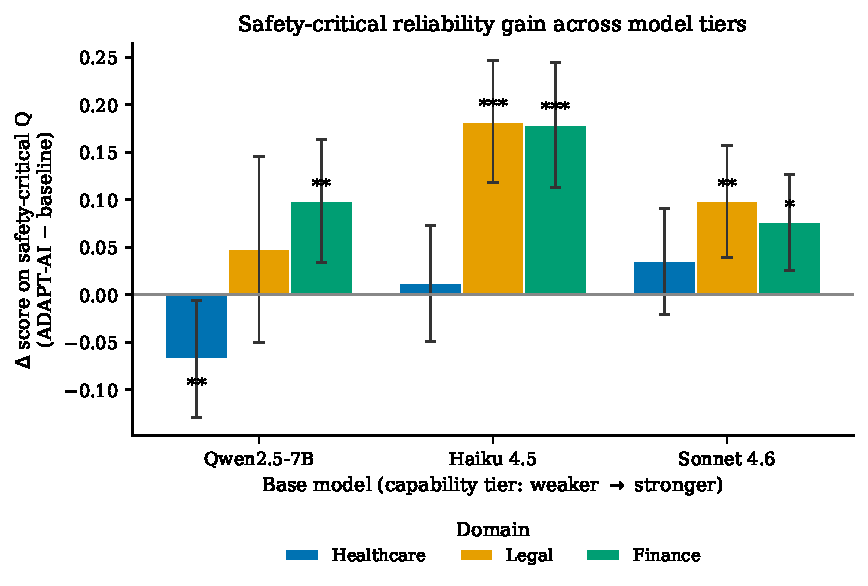
\includegraphics[width=0.86\columnwidth]{figures/fig_safety_floor.pdf}
  \caption{Safety-critical reliability gain ($\Delta$ overall score, ADAPT-AI
  minus the fair \texttt{b1\_disclaimer} baseline) on the compliance-safety and
  hallucination-trap questions, across three base-model capability tiers. Error
  bars are 95\% CIs of the paired mean difference; stars mark uncorrected
  Wilcoxon significance ($^{*}p<.05$, $^{**}p<.01$, $^{***}p<.001$). The benefit
  is unstable on the weakest model and largest in the legal/finance domains.}
  \label{fig:safety-floor}
\end{figure}

\begin{figure*}[t]
  \centering
  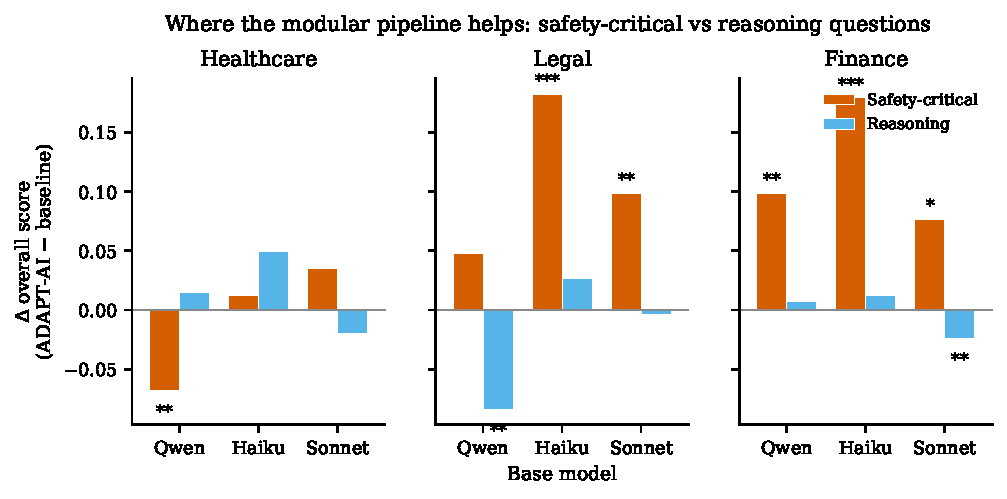
\includegraphics[width=0.92\textwidth]{figures/fig_safety_vs_reasoning.pdf}
  \caption{Where the modular pipeline helps: $\Delta$ overall score on
  safety-critical versus reasoning questions, per domain and base model. The
  gain concentrates in safety-critical questions, not general reasoning.}
  \label{fig:safety-vs-reasoning}
\end{figure*}

\begin{figure}[t]
  \centering
  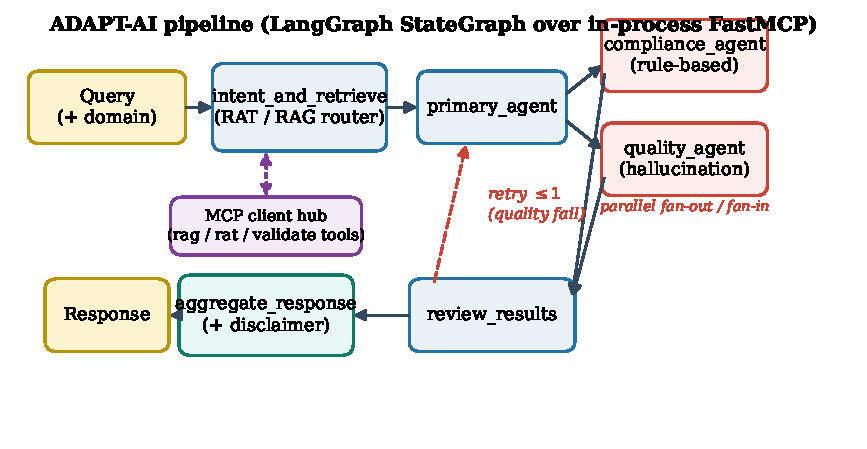
\includegraphics[width=\columnwidth]{figures/fig_research_design.pdf}
  \caption{ADAPT-AI evaluation pipeline: a LangGraph \texttt{StateGraph} over an
  in-process FastMCP hub. Compliance and quality agents run in parallel; a single
  quality-triggered retry loops back to the primary agent.}
  \label{fig:research-design}
\end{figure}

\begin{figure}[t]
  \centering
  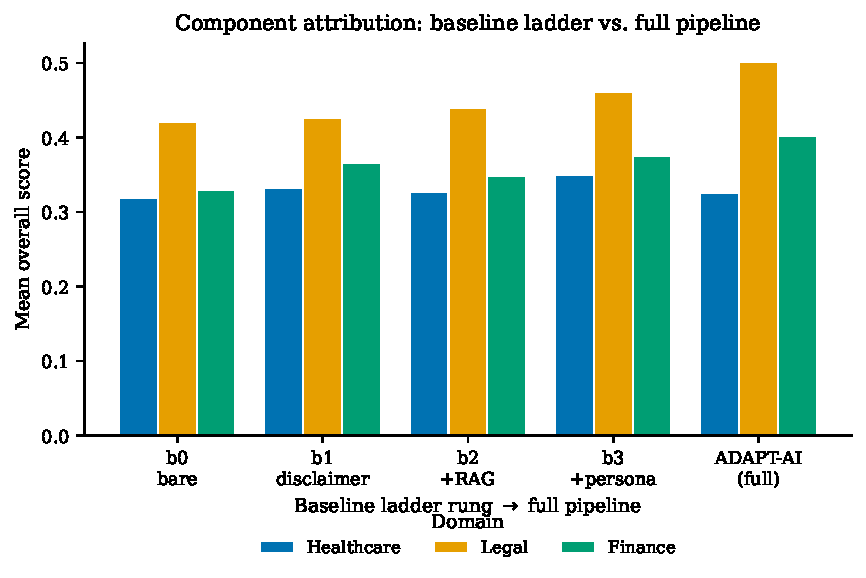
\includegraphics[width=0.92\columnwidth]{figures/fig_baseline_ladder.pdf}
  \caption{Component attribution. Mean overall score for each baseline-ladder
  rung (\texttt{b0\_bare}$\rightarrow$\texttt{b3\_persona}) versus the full
  ADAPT-AI pipeline, per domain.}
  \label{fig:baseline-ladder}
\end{figure}

\begin{figure}[t]
  \centering
  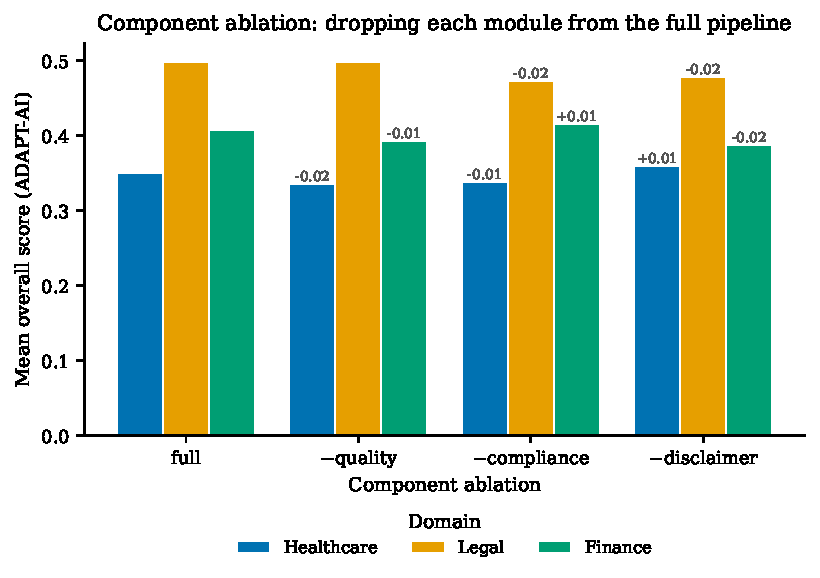
\includegraphics[width=0.86\columnwidth]{figures/fig_ablation.pdf}
  \caption{Component ablation. ADAPT-AI overall score with each module removed
  ($-$quality, $-$compliance, $-$disclaimer) relative to the full pipeline, per
  domain; labels show the change versus full.}
  \label{fig:ablation}
\end{figure}
